\section{Virtualización de un cluster}


En este capitulo se presenta el procedimientos para la virtualización de un Ambiente de Pruebas que simula el funcionamiento de un centro de computación científica con el esquema de Apolo. 

Este proceso es importante para familizarse con el ambiente y los procedimientos en un ambiente seguro, con la posilidad de interacturar con los componentes de manera segura sin afectar de ninguna manera un centro de computo real. 

La siguiente es la descripción de los pasos a seguir para la creación de un ambiente de pruebas paralelo virtualizado que simula el clúster de Apolo.\footnote{Estas instrucciones fueron probadas en un ambiente de Linux Fedora 18.}

\subsection{Requerimientos Mínimos}

\begin{itemize}
	\item Verifique que su computador puede virtualizar: Ingrese a la BIOS y verifique que esta activada la opción de Virtualización de Hardware. 

	\item 3Gb de RAM (o mas)  disponibles para virtualizar.\footnote{1024 RAM para cada Maquina Virtual}
\end{itemize}

\subsection{Configuración del Nodo Maestro}
\begin{enumerate}

\item Descargue e Instale VirtualBox Manager junto con el correspondiente ``Extension Pack'' de la siguiente dirección: \url{https://www.virtualbox.org/wiki/Downloads} \footnote{Tanto la versión de VirtualBox como la versión del ``Extension Pack'' deben coincidir}

	\begin{figure}[H]
		\centering
		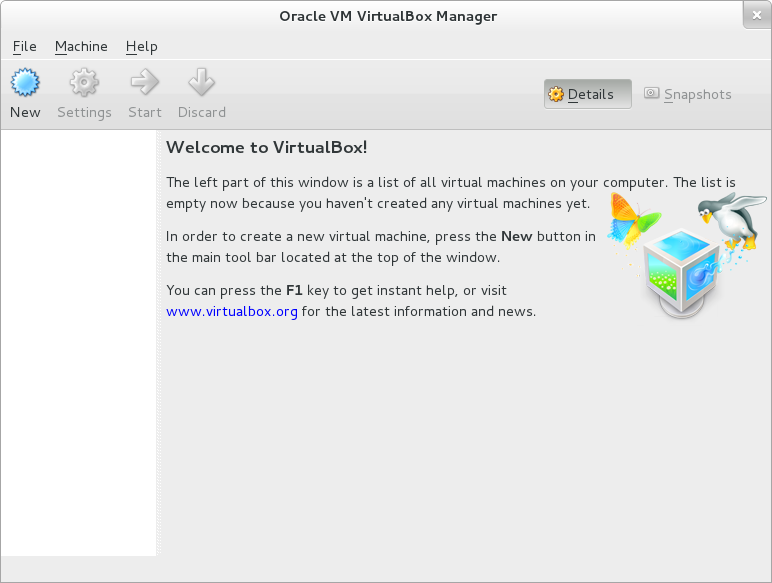
\includegraphics[width=0.5\textwidth]{aux/vb_instalado}
		\caption{Ventana de Virtualbox después de la instalación}
		%(tomada de \cite{WikiEmotion)}
		\label{vb_instalado}
	\end{figure}


\item Descargar la imagen del Master.\footnote{\url{http://goo.gl/8eTJOr}}



\item Una vez instalado VirtualBox en su computador, proceda a instalar el Extensión Pack: 

	
	\begin{figure}[H]
		\centering
		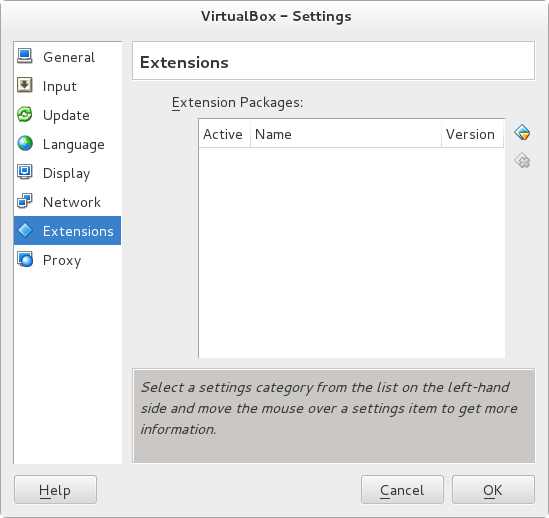
\includegraphics[width=0.5\textwidth]{aux/sinextensionpack}
		\caption{VirtualBox antes de instalar el ``Extension Pack''}
		%(tomada de \cite{WikiEmotion)}
		%\label{F-dimensions-emotion}
	\end{figure}
	
	
\begin{itemize}


	\item En VirtualBox acceda al menú: Archivo $\rightarrow$ Preferencias $\rightarrow$ Sección Extensiones $\rightarrow$ Proceda a instalar el ``Extension Pack''. 
	
	\begin{figure}[H]
		\centering
		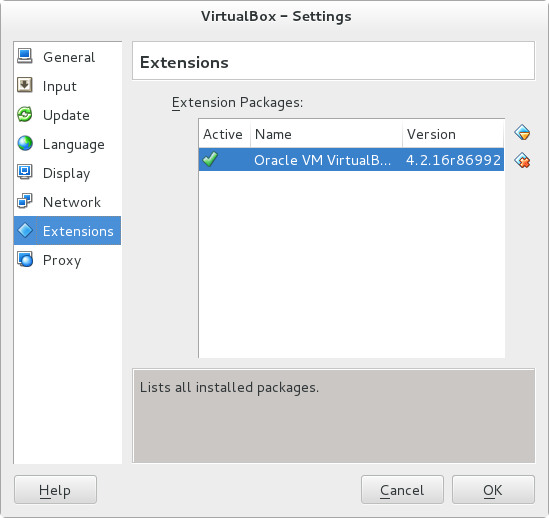
\includegraphics[width=0.5\textwidth]{aux/conextensionpack}
		\caption{Despues de Instalar el ``Extension Pack''}
		%(tomada de \cite{WikiEmotion)}
		%\label{F-dimensions-emotion}
	\end{figure}
	

	\item Vaya a la sección Red $\rightarrow$ Adicione una red Sólo Anfitrión. Asegúrese en caso de tener o crear otra red solo anfitrión que todos los nodos compartan esta red.


	
	\begin{figure}[H]
		\centering
		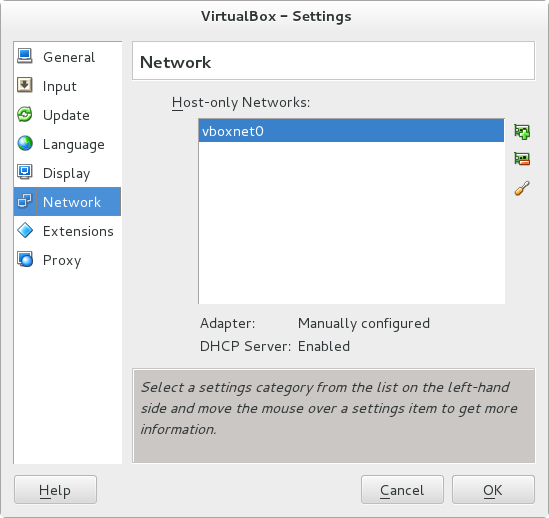
\includegraphics[width=0.5\textwidth]{aux/hostonly}
		\caption{Red Sólo Anfitrion ``vboxnet0''}
		%(tomada de \cite{WikiEmotion)}
		%\label{F-dimensions-emotion}
	\end{figure}
	
	

	\item Haga clic en aceptar para finalizar la operación.

\end{itemize}

\item En VirtualBox, importe desde el Menú $\rightarrow$ Importar Appliance. Deje la configuración por defecto y \textbf{no} reinicialice la dirección MAC.



\begin{figure}[H]
	\centering
	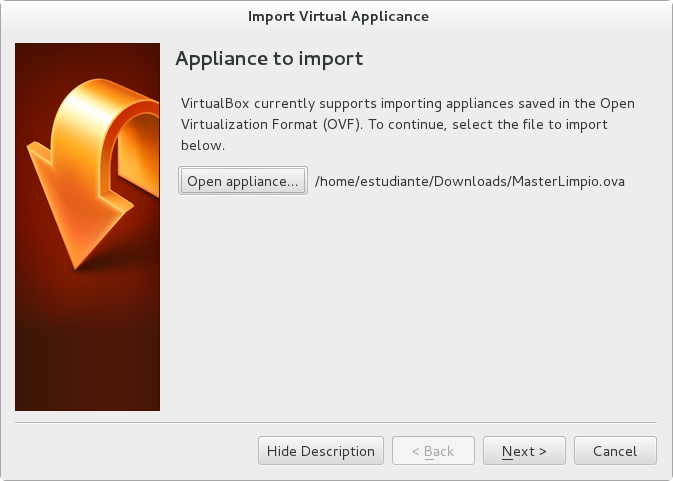
\includegraphics[width=0.5\textwidth]{aux/importappliance}
	\caption{Importar Maquina Virtual}
	%(tomada de \cite{WikiEmotion)}
	%\label{F-dimensions-emotion}
\end{figure}


\begin{figure}[H]
	\centering
	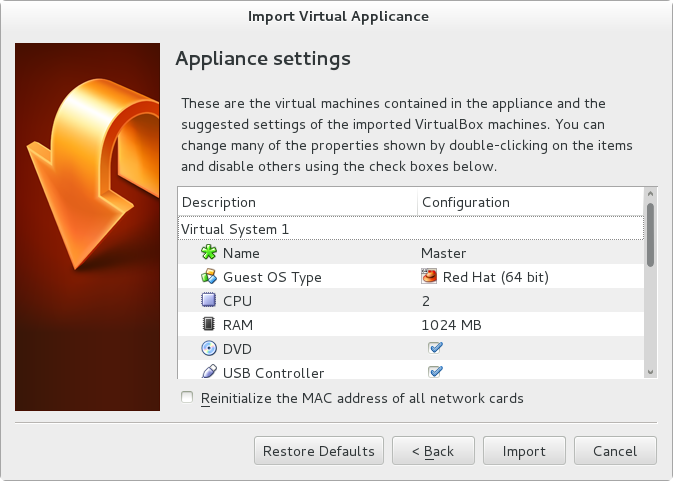
\includegraphics[width=0.5\textwidth]{aux/applianceops1}
	\caption{Opciones de configuración de la Maquina Virtual}
	%(tomada de \cite{WikiEmotion)}
	%\label{F-dimensions-emotion}
\end{figure}


\begin{figure}[H]
	\centering
	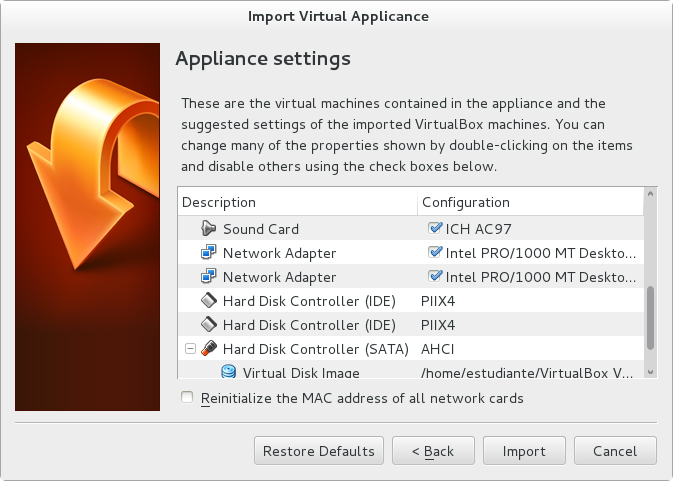
\includegraphics[width=0.5\textwidth]{aux/applianceops2}
	\caption{Más opciones de configuración de la Maquina Virtual}
	%(tomada de \cite{WikiEmotion)}
	%\label{F-dimensions-emotion}
\end{figure}



\item Seleccione la máquina virtual llamada ``Master'' y vaya a la configuración y revise la siguiente configuración en esta:

\begin{itemize}

	\item En la sección Sistema, pestaña Procesador, debe tener dos procesadores y habilitado PAE/NX.

	
	
	
	\begin{figure}[H]
		\centering
		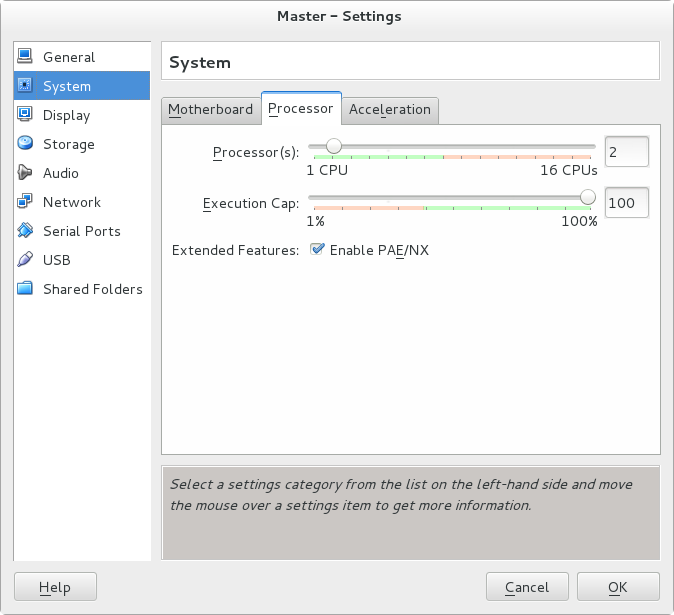
\includegraphics[width=0.5\textwidth]{aux/procesadores}
		\caption{Procesadores e Inicio por PAE/NX}
		%(tomada de \cite{WikiEmotion)}
		%\label{F-dimensions-emotion}
	\end{figure}
	
	

	\item En la sección Red, pestaña Adaptador 1, deberá estar configurado como NAT. 


	
	\begin{figure}[H]
		\centering
		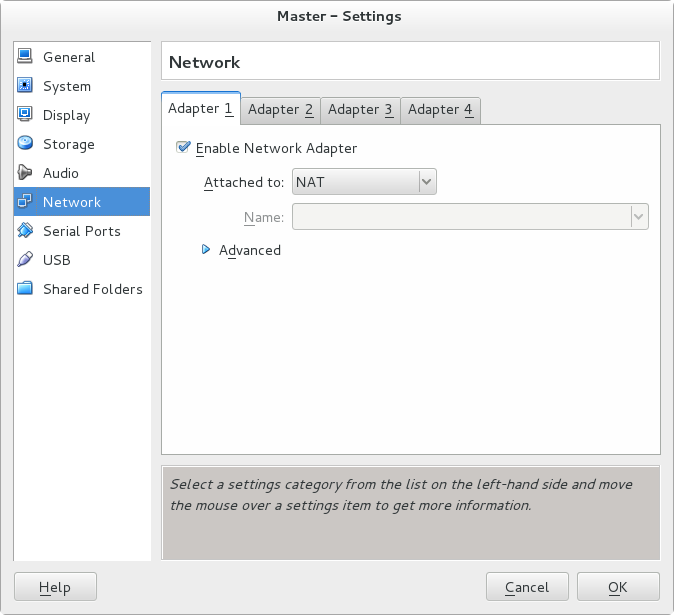
\includegraphics[width=0.5\textwidth]{aux/rednat}
		\caption{Configuración Red Adaptador 1: NAT}
		%(tomada de \cite{WikiEmotion)}
		%\label{F-dimensions-emotion}
	\end{figure}
	
	

	\item En la pestaña Adaptador 2 deberá estar en Adaptador Sólo--Anfitrión y el nombre deberá ser \texttt{vboxnet0}\footnote{Tenga en cuenta que este adaptador se llama \texttt{vboxnet0} en Linux, en Windows tendrá otro nombre, lo más importante es que sea la misma interfaz de red de Sólo Anfitrión, ya que sino dará lugar al problema de reasignación de interfaces de red dentro del nodo Master, en otras palabras, asignará las interfaces eth2 y eth3 en vez de asignar eth0 y eth1 a la NAT y a la Sólo Anfitrión respectivamente.}.


	
	\begin{figure}[H]
		\centering
		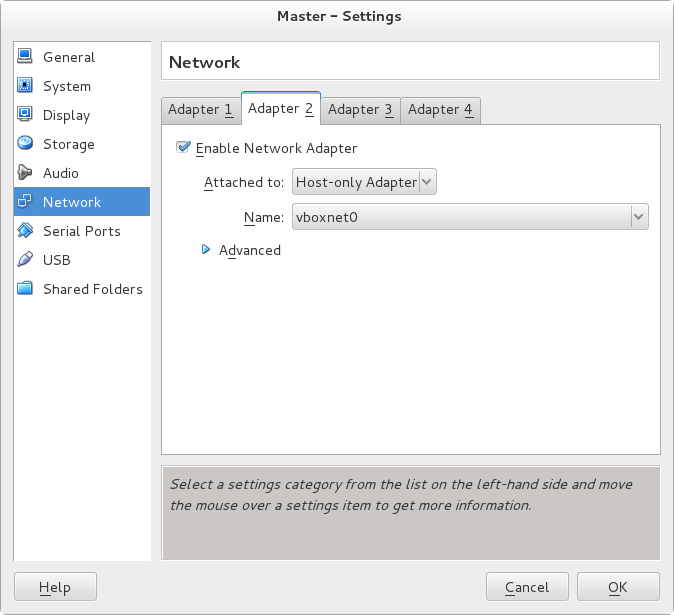
\includegraphics[width=0.5\textwidth]{aux/redhost}
		\caption{Red Host Only (Sólo Anfitrión)}
		%(tomada de \cite{WikiEmotion)}
		%\label{F-dimensions-emotion}
	\end{figure}
	
	

	\item Acepte todos los cambios.

\end{itemize}

\item Seleccione la máquina Master e iníciela.

\item Una vez iniciada la máquina virtual del Master proceda a crear una nueva máquina virtual como Nodo Trabajador a partir de los siguientes pasos:

\begin{itemize}
	\item Haga clic en Crear Nueva Máquina.

	\item El nombre será \texttt{compute-0-0}.

	\item El tipo será Linux.

	\item La versión será Red Hat de 64 bits.

	
	\begin{figure}[H]
		\centering
		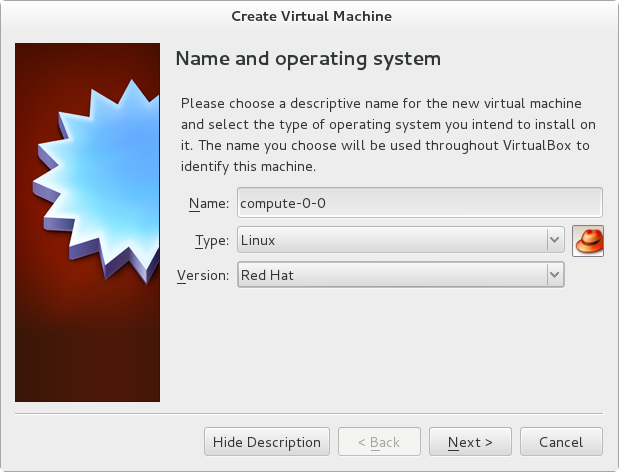
\includegraphics[width=0.5\textwidth]{aux/opcnodo1}
		\caption{Opciones para el compute-0-0}
		%(tomada de \cite{WikiEmotion)}
		%\label{F-dimensions-emotion}
	\end{figure}
	
	\item Clic en siguiente.

	\item Asigne 1024 Megabytes de Memoria RAM\footnote{La cantidad de memoria RAM asignada será proporcional a la que tenga el sistema en el cual están las máquinas virtuales. Igual con el disco duro y los procesadores, sin embargo, para efectos de ver la paralelización en memoria compartida se recomienda tener 2 procesadores por máquina}.

	\item Cree el disco duro con 30 gigas de espacio, recuerde que esto se asignará dinámicamente. El tipo de disco duró será VDI y dinámicamente asignado.



	
	\begin{figure}[H]
		\centering
		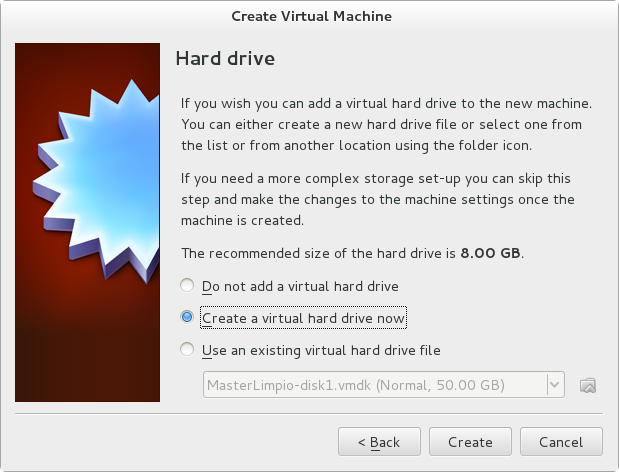
\includegraphics[width=0.5\textwidth]{aux/nodohd}
		\caption{Crear un Nuevo Disco Virtual (VHD)}
		%(tomada de \cite{WikiEmotion)}
		%\label{F-dimensions-emotion}
	\end{figure}
	

	
	
	\begin{figure}[H]
		\centering
		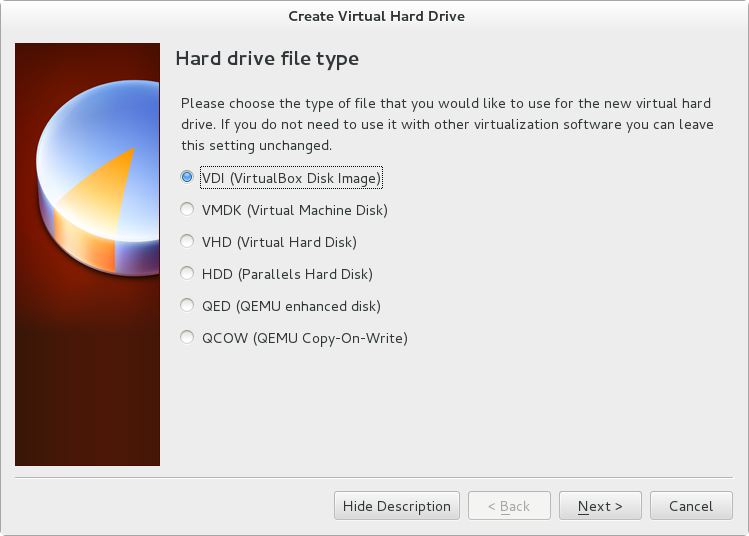
\includegraphics[width=0.5\textwidth]{aux/nododvi}
		\caption{Tipo de disco a crear}
		%(tomada de \cite{WikiEmotion)}
		%\label{F-dimensions-emotion}
	\end{figure}
	


	
	\begin{figure}[H]
		\centering
		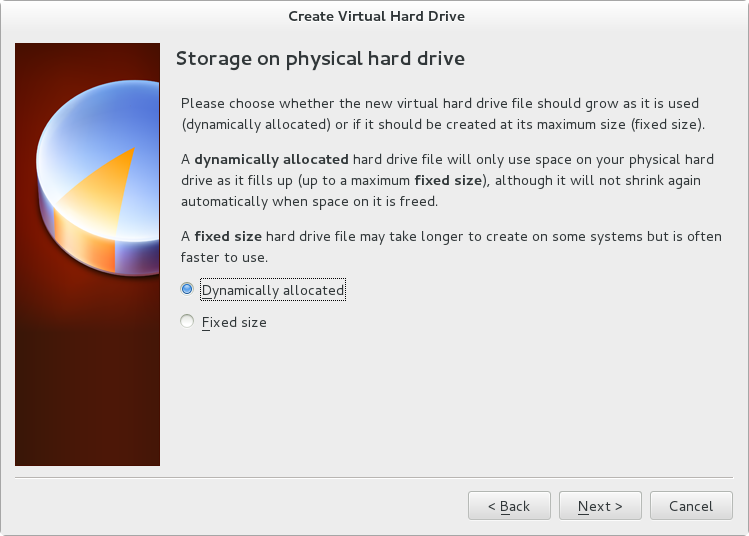
\includegraphics[width=0.5\textwidth]{aux/hddinamico}
		\caption{Opciones para Disco Dinámico o Estático}
		%(tomada de \cite{WikiEmotion)}
		%\label{F-dimensions-emotion}
	\end{figure}
	



	\begin{figure}[H]
		\centering
		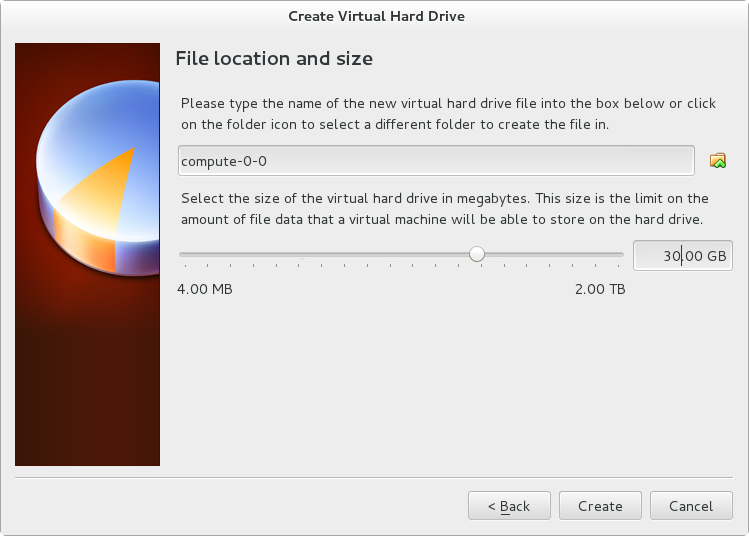
\includegraphics[width=0.5\textwidth]{aux/nodohdsize}
		\caption{Tamaño del Disco}
		%(tomada de \cite{WikiEmotion)}
		%\label{F-dimensions-emotion}
	\end{figure}
		

\end{itemize}

\item Una vez creado el nodo trabajador se procede a configurarlo a partir de los siguientes pasos:

\begin{itemize}
	\item Señalar la máquina \texttt{compute-0-0} y dar clic en Configurar.

	\item En la pestaña Sistema, asegúrese de que tenga la cantidad de memoria RAM correcta

	\item Deshabilite el \texttt{floppy disk}

	\item habilite la red como dipositivo de \texttt{booteo} y además súbalo como primer dispositivo, sólo deberá quedar la tarjeta de red como primera opción y como segunda el disco duro de la máquina virtual, de esta manera nos aseguramos que esta máquina virtual pueda instalarse automáticamente de manera desatendida, por esta razón el clúster es escalable. 

	
	\begin{figure}[H]
		\centering
		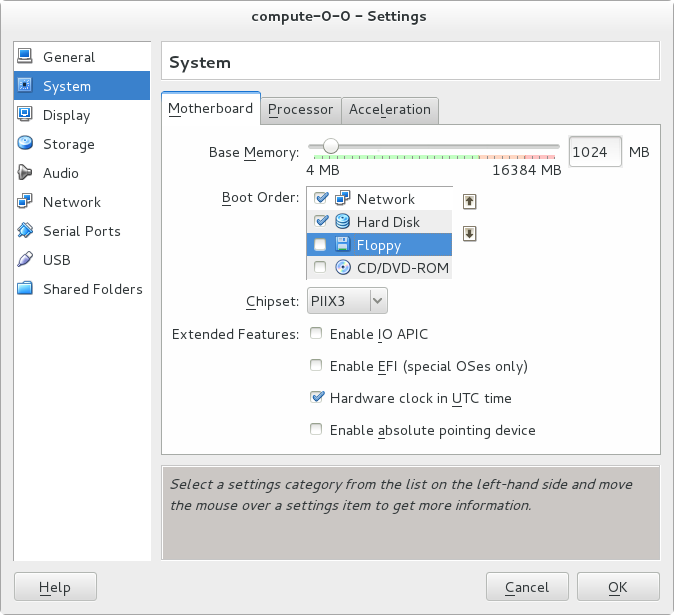
\includegraphics[width=0.5\textwidth]{aux/nodoopsboot}
		\caption{Opciones del Nodo }
		%(tomada de \cite{WikiEmotion)}
		%\label{F-dimensions-emotion}
	\end{figure}
	


	\item En la pestaña Procesador asegúrese de que hay dos procesadores y está habilitado PAE/NX.



	\begin{figure}[H]
		\centering
		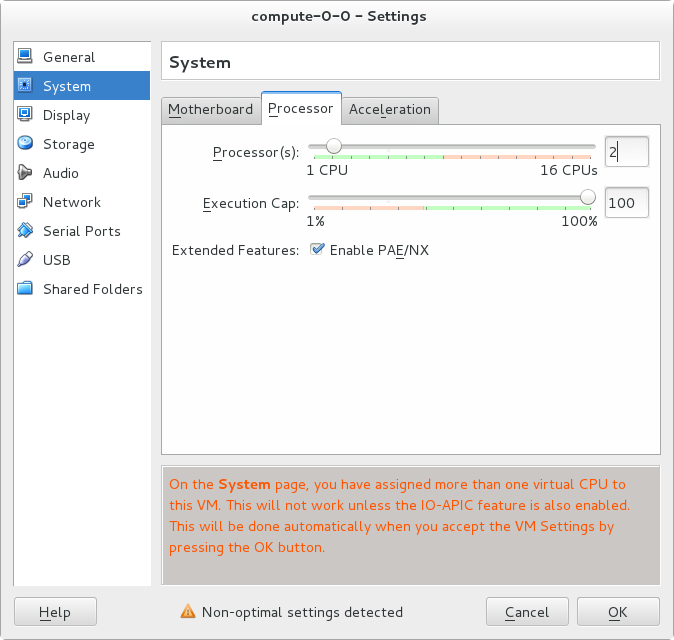
\includegraphics[width=0.5\textwidth]{aux/nodoprocesadores}
		\caption{Opciones Procesador para el Nodo}
		%(tomada de \cite{WikiEmotion)}
		%\label{F-dimensions-emotion}
	\end{figure}
		

	\item En la sección Red deberá configurar sólo la primera interfaz de red y deberá estar configurada como Sólo--Anfitrión y deberá tener \texttt{vboxnet0}.


	
	\begin{figure}[H]
		\centering
		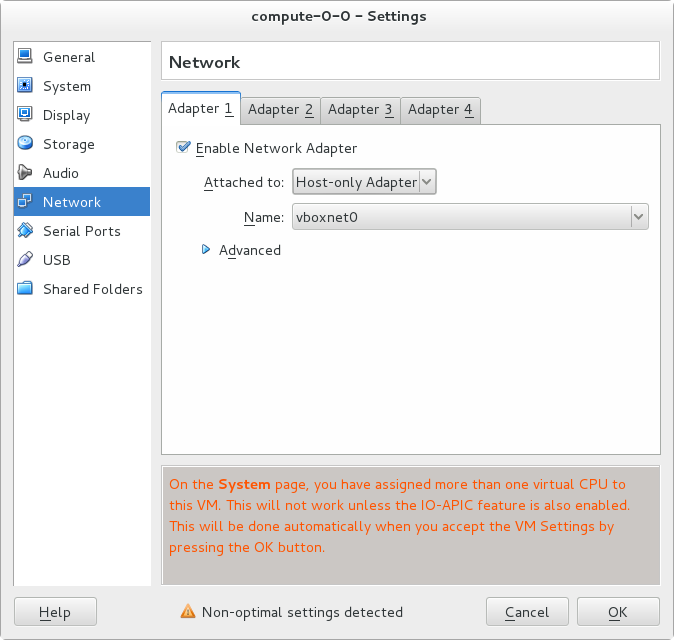
\includegraphics[width=0.5\textwidth]{aux/nodored}
		\caption{Opciones de Red del Nodo}
		%(tomada de \cite{WikiEmotion)}
		%\label{F-dimensions-emotion}
	\end{figure}
	
	

	\item Acepte los cambios.
\end{itemize}


\item Repita los pasos para crear otro nodo si lo considera necesario para crear el \texttt{compute-0-1}, siempre y cuando la computadora que usted tiene soporte una tercera máquina virtual ejecutandose al tiempo que el Nodo Master y el \texttt{compute-0-0}

\item Ingrese en el Nodo Master como usuario \texttt{root} y la contraseña es \texttt{apolito123!}

\item Abra una consola (La combinación de teclas Alt+F2 permite ejecutar una aplicación escribiendo su nombre)



\begin{figure}[H]
	\centering
	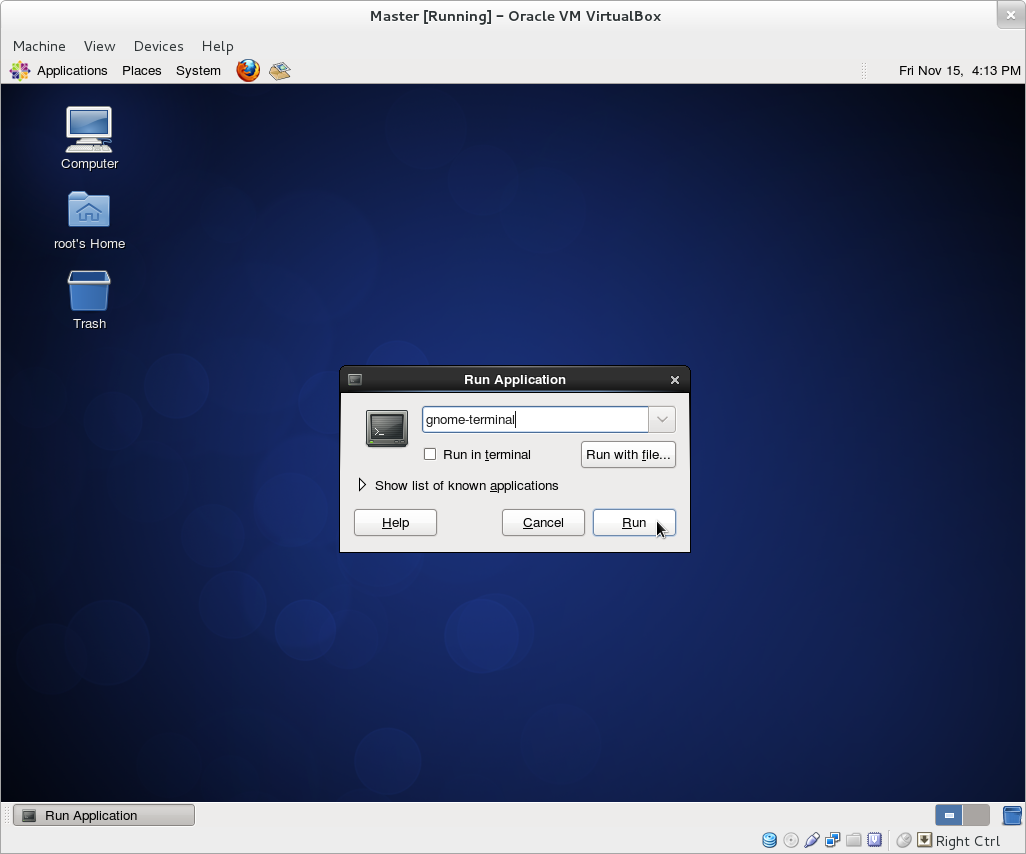
\includegraphics[width=0.5\textwidth]{aux/terminal}
	\caption{Abrir Terminal}
	%(tomada de \cite{WikiEmotion)}
	%\label{F-dimensions-emotion}
\end{figure}



\item Ingrese el comando \texttt{insert-ethers}



\begin{figure}[H]
	\centering
	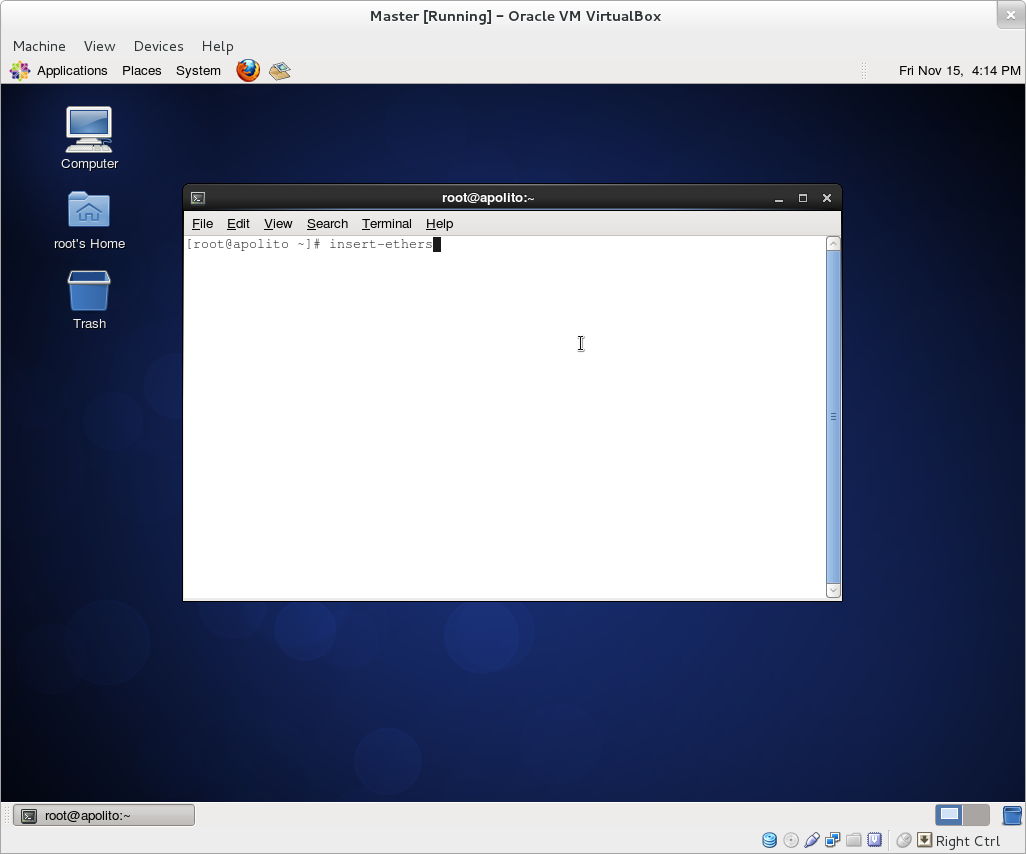
\includegraphics[width=0.5\textwidth]{aux/insert}
	\caption{Captura de los nodos por parte del Master}
	%(tomada de \cite{WikiEmotion)}
	%\label{F-dimensions-emotion}
\end{figure}



\item Escoja \texttt{Compute}. Aparecerá una interfaz de consola mostrándole los nodos agregados en la medida que se les vaya asignando IP por medio de DHCP y una imagen de Linux para instalar con PXE.



\begin{figure}[H]
	\centering
	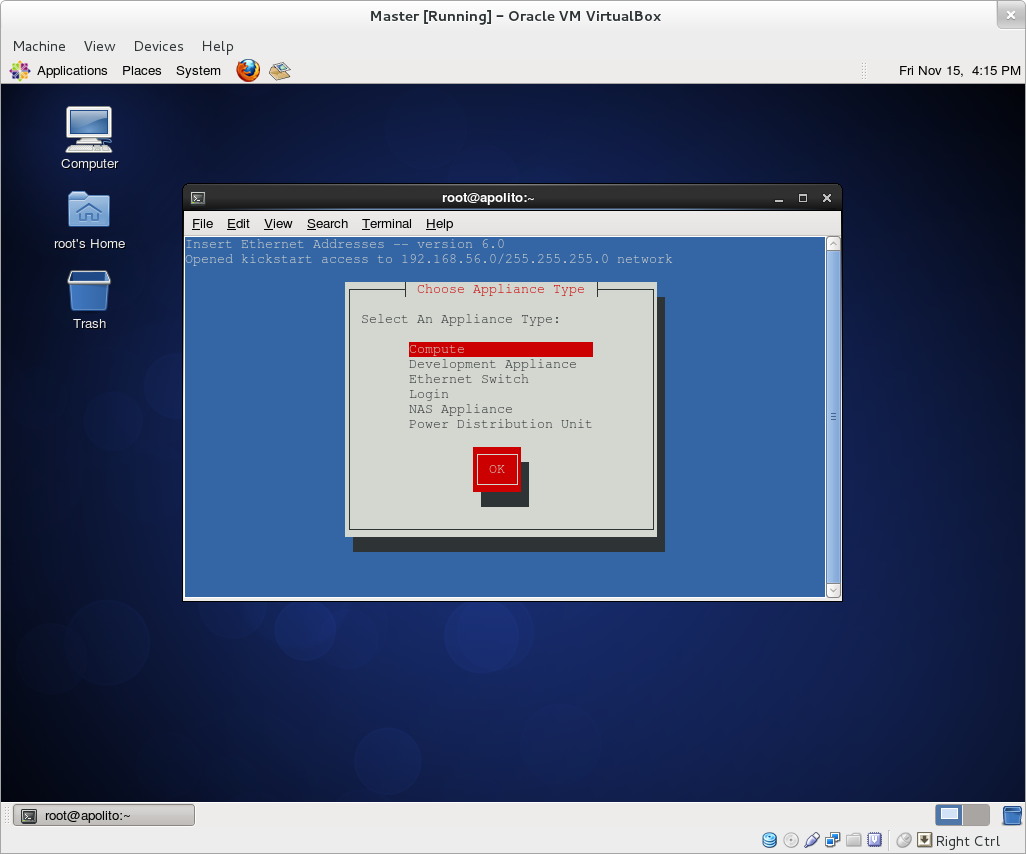
\includegraphics[width=0.5\textwidth]{aux/compute}
	\caption{inserción de los Nodos tipo ``Compute''}
	%(tomada de \cite{WikiEmotion)}
	%\label{F-dimensions-emotion}
\end{figure}



\item Encienda de uno en uno los Nodos trabajadores que haya creado, empezando por el \texttt{compute-0-0} y así sucesivamente. Observará que aparece en la interfaz \texttt{insert-ethers} la dirección MAC del Nodo Trabajador, se le asignará el nombre compute-0-0 y si aparece un símbolo de asterisco es porque recibió exitosamente la imagen para la instalación de Linux.




\begin{figure}[H]
	\centering
	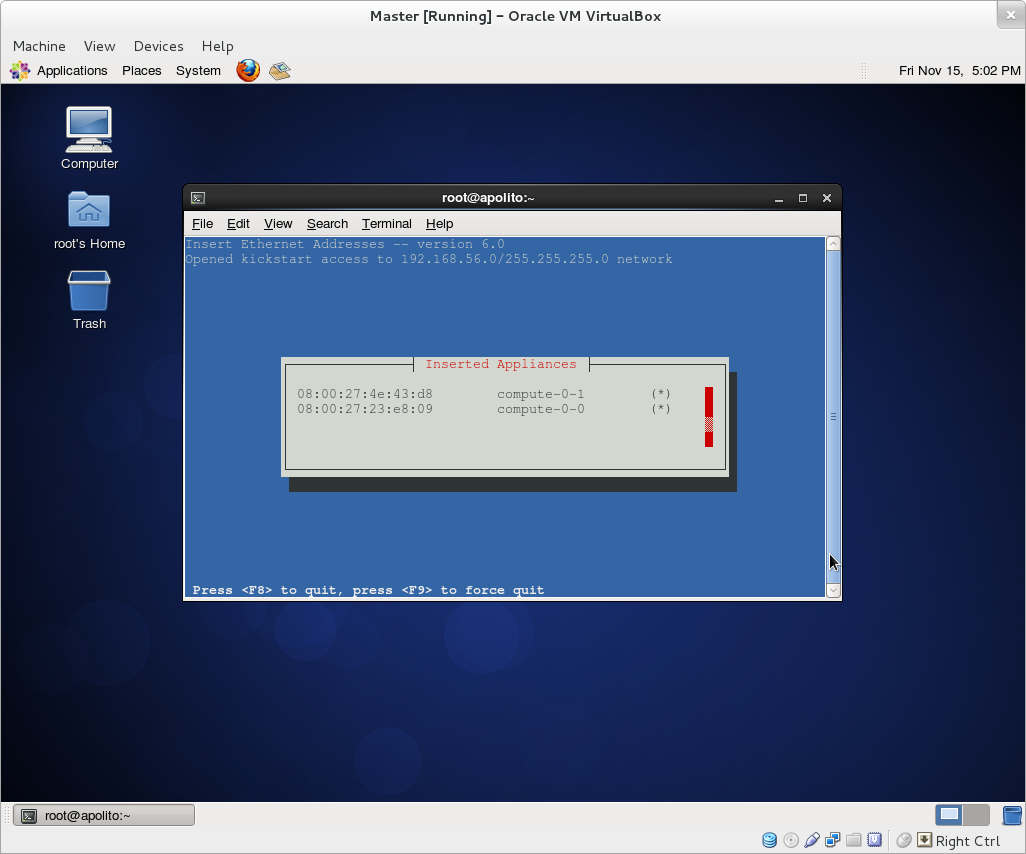
\includegraphics[width=0.5\textwidth]{aux/nodosinsertados}
	\caption{Nodos ya reconocidos por el master}
	%(tomada de \cite{WikiEmotion)}
	%\label{F-dimensions-emotion}
\end{figure}



\item Una vez de que los nodos se termine de instalar automáticamente salga de la interfaz de \texttt{insert-ethers} en el Master con la tecla F8.

\item Ingrese al directorio especificado con el siguiente comando: \texttt{cd /export/apps/installers}

\item Descargue el instalador del comando \texttt{htop} con la siguiente instrucción: \texttt{wget http://goo.gl/TDWExw}

\item Instale \texttt{htop} en el nodo Master con la siguiente instrucción: \texttt{rpm -ivh htop*.rpm}

\item Ahora instale masivamente \texttt{htop} en el resto del clúster con el siguiente comando: \texttt{rocks run host ``rpm -ivh /share/apps/installers/htop*.rpm''}

\item El cluster está completo.

\end{enumerate}

\subsection{Configuración de los Nodos Esclavos}

\begin{enumerate}
	\item Una vez que se tiene el nodo Master funcionando y por lo menos un nodo trabajador como el \texttt{compute-0-0} se procede a realizar los siguientes pasos de configuración:

	\begin{itemize}
	\item Adicione un usuario sin privilegios con los siguientes comandos\footnote{En adelante el usuario de ejemplo será smonsalve, pero usted podrá asignar el nombre de usuario que desee}:

	\begin{itemize}
		\item \textbf{\texttt{adduser smonsalve}} Para crear un usuario sin privilegios.

		\item \textbf{\texttt{passwd smonsalve}} Para cambiar la contraseña del usuario.

		\item \textbf{\texttt{rocks sync users}} Para sincronizar el usuario creado en todo el cluster, este usuarió estará creado tanto en el nodo master como en los nodos trabajadores.
	\end{itemize}

	\item \texttt{su - smonsalve} Para que pasemos de estar con el usuario \texttt{root} y estemos con en el usuario sin privilegios. Se le harán algunas preguntas de contraseñas, puede llenarlas o déjelas vacías y continuar presionando la tecla \texttt{enter} varias veces.
	\end{itemize}
	
\end{enumerate}

\subsection{Apagar el Clúster}

Cada vez que se vaya a apagar el ambiente de Pruebas es necesario realizarlo con el siguiente procedimiento para evitar dañar la configuración de los nodos. 

\begin{itemize}
	\item Desde una consola en el master ejecutar el siguiente comando que le indicara los respectivos nodos que se apaguen de manera adecuada. 

	 \begin{verbatim}
	$ rocks run host poweroff
 	\end{verbatim}

 	\item 
  
\end{itemize}







\section{Preguntas Frecuentas:}[Posibles Problemas]

\begin{itemize}
	\item Los nodos de trabajo no inician Correctamente: Es posible que estos hayan sido apagados de manera incorrecta. 
	siga el procedimiento desde el numeral X hasta el Y de ``ASDF''

	\item 
	\item Si su caso no se encuentra aquí listado contacte al autor
\end{itemize}




